\section{Event selection, mass resolution, and radiative fraction}
\label{sec:event-selection}

Each HPS input is an invariant-mass spectrum formed after a run-specific event
selection. That selection determines the composition of the prompt $e^+e^-$ sample;
the detector response sets the width of a possible resonance, and the radiative
fraction sets its normalization. Together, these ingredients connect the recorded
events to the signal model used in the search.

\subsection{Prompt event selection}

Across the three HPS campaigns, the prompt selection follows the same experimental
logic:
oppositely charged tracks matched to ECal clusters, tight cluster-time coincidence,
track-quality and vertex-reconstruction requirements, and momentum cuts that retain
prompt radiative tridents while suppressing accidentals and converted wide-angle
bremsstrahlung. The 2015 and 2016 selections are inherited from the published prompt
searches. For 2021 we use the prompt target-constrained (prompt-TC) sample summarized in
Table~\ref{tab:event-selection}. It requires
$p_{\mathrm{sum}}>\SI{2.8}{GeV}$ and applies no additional vertex-fit $\chi^2$
requirement. The stored hit count is three-dimensional and does not document a separate
eight-hit two-dimensional electron requirement, so we do not include one here.

In Table~\ref{tab:event-selection}, $V_0$ denotes a reconstructed $e^+e^-$ vertex,
GBL is the track-fit algorithm, FEE denotes the full-energy-electron veto, and TC means
target constrained. Pair1, Single-2, and Single-3 are the trigger names used during the
corresponding data-taking periods.

\begingroup
\small
\setlength{\tabcolsep}{3pt}
\begin{longtable}{@{}P{0.15\linewidth} P{0.27\linewidth} P{0.27\linewidth} P{0.27\linewidth} @{}}
\caption{Comparison of the prompt-resonance selections. The 2015 and 2016 columns
follow the published and internal engineering-run summaries. For 2021, the
preselection entries follow the full analysis note
\cite[Sec.~4.8 and App.~A]{HPS2021FullAnalysisNote}; the prompt entries list the
additional requirements documented for the native 10\% prompt-TC sample.}
\label{tab:event-selection}\\
\toprule
\textbf{Cut type} &
\textbf{2015 (Eng. run 1)} &
\textbf{2016 (Eng. run 2)} &
\textbf{2021 (native 10\%)} \\
\midrule
\endfirsthead

\toprule
\textbf{Cut type} &
\textbf{2015 (Eng. run 1)} &
\textbf{2016 (Eng. run 2)} &
\textbf{2021 (native 10\%)} \\
\midrule
\endhead

\bottomrule
\endfoot

\bottomrule
\endlastfoot

Trigger / topology &
\Pre pairs-1 trigger; ECAL halves:\newline
$y_{e^+}^{\rm clu}y_{e^-}^{\rm clu}<0$.\newline
\Pro same. &
	\Pre Pair1 trigger bit; opposite ECal halves; the trigger does not encode track
	charge.\newline
\Pro same. &
\Pre Single-2 or Single-3 positron single-cluster trigger; Single-3 also requires the
matched hodoscope condition used by the 2021 trigger menu.\newline
\Pro no additional prompt-TC requirement. \\

Track momenta &
\Pre $p(e^-)<0.75\,E_{\rm beam}$.\newline
\Pro $p_{\rm sum}>0.8\,E_{\rm beam}$ and $p_{\rm sum}<1.2\,E_{\rm beam}$. &
\Pre $p(e^\pm)<2.15~\mathrm{GeV}$; $p_{\rm sum}<1.2\,E_{\rm beam}$.\newline
\Pro $p_{\rm sum}>1.90~\mathrm{GeV}$ and $p_{\rm sum}<2.4~\mathrm{GeV}$. &
\Pre $p_{\rm trk}>0.4~\mathrm{GeV}$ for each track; FEE veto
$p(e^-)<2.9~\mathrm{GeV}$; vertex momentum $p_{\rm vtx}<4.0~\mathrm{GeV}$.\newline
\Pro the prompt-TC sample requires $p_{\rm sum}>2.8~\mathrm{GeV}$. \\

Track fit / hits &
\Pre loose track--cluster match:
$\chi^2_{\rm trk-clu}<10$.\newline
\Pro GBL track $\chi^2_{\rm trk}<40$. &
\Pre $\chi^2_{\rm trk}<12$; PID goodness $<10$.\newline
\Pro no additional prompt requirement is documented. &
\Pre $\chi^2_{\rm trk}/{\rm ndf}<20$ and $N_{\rm 2D~hits}\ge10$ for the tracks.\newline
\Pro no additional 2D-hit requirement is established; the available field counts
3D hits. \\

Track--cluster timing &
\Pre ---\newline
\Pro $|t_{\rm clu}-t_{\rm trk}-43~\mathrm{ns}|<4.5~\mathrm{ns}$. &
\Pre $|t_{\rm trk}-t_{\rm clu}|<6~\mathrm{ns}$.\newline
\Pro no additional value stated. &
\Pre full-note data timing windows:
$\Delta(t_{e^-,{\rm trk}},t_{e^+,{\rm clu}})<6.0~\mathrm{ns}$,
$\Delta(t_{e^+,{\rm trk}},t_{e^+,{\rm clu}})<5.1~\mathrm{ns}$, and
$\Delta(t_{e^-,{\rm trk}},t_{e^+,{\rm trk}})<7.8~\mathrm{ns}$.\newline
\Pro no additional prompt-TC timing requirement. \\

Cluster--cluster coincidence &
\Pre ---\newline
\Pro $|\Delta t_{\rm clu-clu}|<2~\mathrm{ns}$. &
\Pre $|\Delta t_{\rm clu-clu}|<2~\mathrm{ns}$.\newline
\Pro $|\Delta t_{\rm clu-clu}|<1.43~\mathrm{ns}$. &
\Pre no separate offline cluster--cluster coincidence appears in the full preselection
table; the Pair-0 hardware trigger has a cluster-pair timing window
$|\Delta t|<12~\mathrm{ns}$ and VTP prescale 100.\newline
\Pro no additional prompt-TC offline coincidence requirement. \\

Vertex / $V_0$ quality &
\Pre if multiple $V_0$ remain, choose the best $\chi^2_{\rm vtx}$.\newline
\Pro $\chi^2_{\rm vtx}<75$ and $p(V_0)<1.2\,E_{\rm beam}$. &
\Pre target-constrained $V_0$ candidates.\newline
\Pro no additional prompt $\chi^2_{\rm vtx}$ requirement is documented. &
\Pre full-note upgraded-detector values:
$p_{\rm vtx}<4.0~\mathrm{GeV}$ and $\chi^2_{\rm vtx}<20$.\newline
\Pro no additional prompt-TC vertex-fit $\chi^2$ requirement. \\

Positron cluster energy &
\Pre ---\newline \Pro --- &
\Pre ---\newline \Pro --- &
\Pre full-note sanity cut $E^{\rm clu}_{e^+}>0.2~\mathrm{GeV}$.\newline
\Pro no additional prompt-TC positron-cluster threshold. \\

cWAB suppression &
\Pre ---\newline
\Pro $e^+$ must have L1 and L2 hits; $d_0(e^+)<1.1~\mathrm{mm}$; and
$(p_T^- - p_T^+) / (p_T^- + p_T^+) < 0.47$. &
\Pre ---\newline
\Pro not applied in the final 2016 prompt selection summary. &
\Pre no explicit cWAB-suppression cut is listed in the full 2021 preselection table.\newline
\Pro no additional prompt-TC cWAB requirement. \\

Candidate multiplicity &
\Pre unique-$V_0$ policy: keep the best $\chi^2_{\rm vtx}$.\newline
\Pro enforced by the unique-$V_0$ logic. &
\Pre ---\newline
\Pro require a single surviving $V_0$ candidate. &
\Pre exactly one selected good vertex: $N_{\rm vtx}>0$ and $N_{\rm vtx}<2$.\newline
\Pro no additional prompt-TC multiplicity requirement. \\
\end{longtable}
\endgroup




The 2021 preselection entries follow the full analysis note
\cite[Sec.~4.8 and App.~A]{HPS2021FullAnalysisNote}.
\ifwritingsample
The native 10\% spectrum comes from the prompt-TC sample. The GPR fit adds no
event-level cuts.
\else
The complete-note build reads the native 10\% mass spectrum preselection/h\_invM\_8000 from a
hash-bound ROOT input whose recorded SHA-256 matches final\_10pct\_invM.root. The GPR
fit adds no event-level cuts.
\fi
Each campaign enters the analysis through its selected invariant-mass histogram and
the detector-response and normalization inputs for the same event category.

The engineering-run notes use \emph{preselection} for the broad reconstruction sample
and \emph{prompt selection} for the tighter resonance-search sample. The 2021 input is
closer to the latter because the prompt-TC sample retains the high-$p_{\mathrm{sum}}$
side. Table~\ref{tab:event-selection} keeps that distinction without adding an
unrecorded two-dimensional hit requirement.

\ifwritingsample
\else
% ============================================================
%  Preselection validation figures (v13 signal overlay)
% ============================================================
The 2021 preselection figures below show selected reconstruction variables. The signal
simulation has an arbitrary normalization, so only the distribution shapes can be
compared, not yields or efficiencies.

% ------------------------------------------------------------
%  4. Vertex quantities
% ------------------------------------------------------------
% The reconstructed-vertex observables are shown in
% Figure~\ref{fig:presel_vertex}: the vertex-fit $\chi^2$, the invariant mass,
% and the longitudinal vertex position $V_z$. The vertex $z$ distribution is the
% primary discriminant for the displaced-vertex signal, whose long lifetime
% populates the downstream tail well beyond the prompt data.
\begin{figure}[htbp]
  \centering
  \begin{subfigure}[t]{0.48\textwidth}
    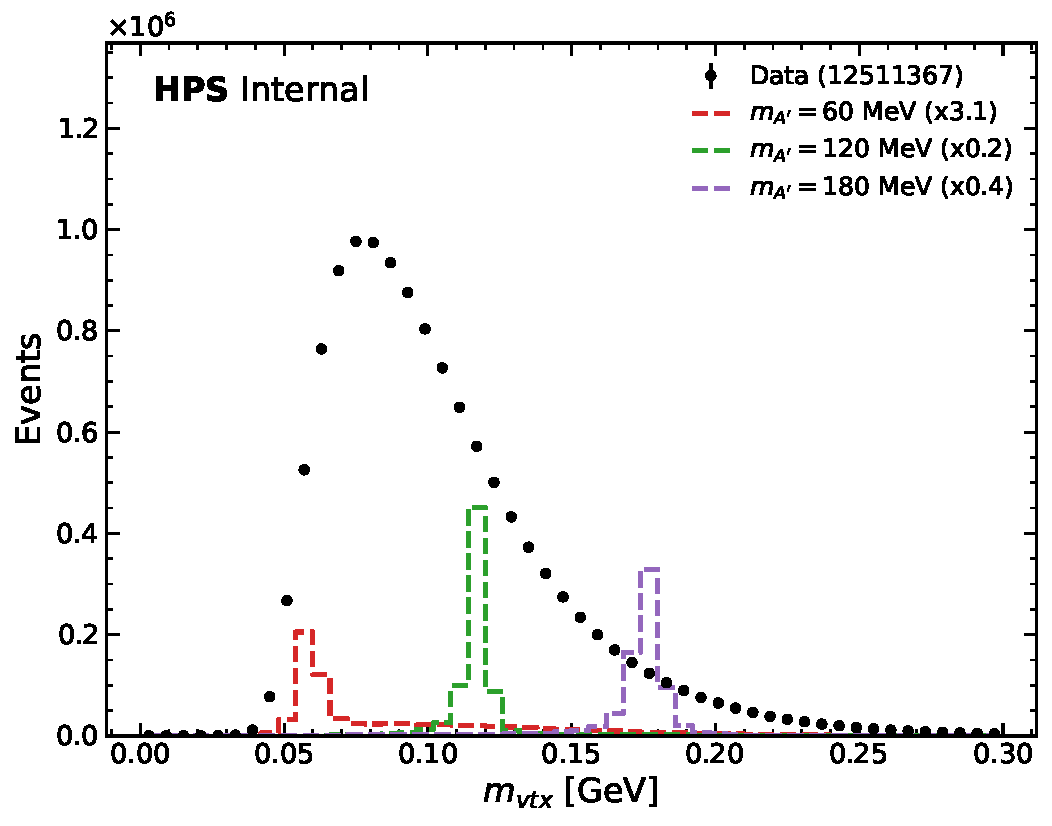
\includegraphics[width=\textwidth]{preselection_plots/signal_overlay_loose_loose_vtx_mass.pdf}
    \caption{Vertex invariant mass.}
  \end{subfigure}\hfill
  \begin{subfigure}[t]{0.48\textwidth}
    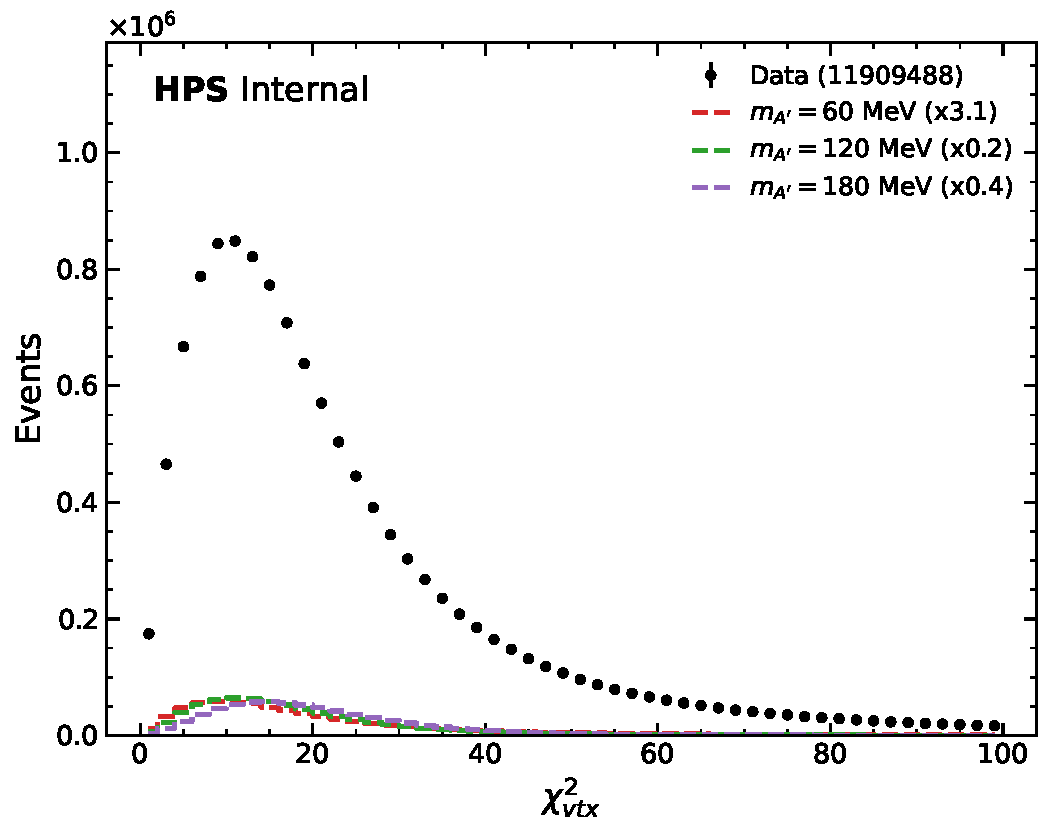
\includegraphics[width=\textwidth]{preselection_plots/signal_overlay_loose_loose_vtx_chi2.pdf}
    \caption{Vertex-fit $\chi^2$.}
  \end{subfigure}
  \caption{Reconstructed-vertex distributions after the loose preselection,
    comparing data (points) with the signal MC (filled histogram). The vertex-fit
    $\chi^2$ is shown as a diagnostic; no vertex-fit $\chi^2$ requirement is applied to
    the regenerated 2021 GPR input.}
  \label{fig:presel_vertex}
\end{figure}

% ------------------------------------------------------------
%  1. Electron track kinematics
% ------------------------------------------------------------
% The following figures compare the loose-preselected data (points) with the
% signal Monte Carlo (histogram), normalised to unit area, for the kinematic
% variables entering the preselection. Figure~\ref{fig:presel_ele_kin} shows the
% electron-track quantities: the total and longitudinal momentum together with
% the transverse and longitudinal impact parameters. Good agreement between the
% shapes of the reconstructed distributions is expected in the bulk of phase
% space, while the signal is characterised by its harder momentum spectrum and
% displaced-vertex tails.
\begin{figure}[htbp]
  \centering
  \begin{subfigure}[t]{0.48\textwidth}
    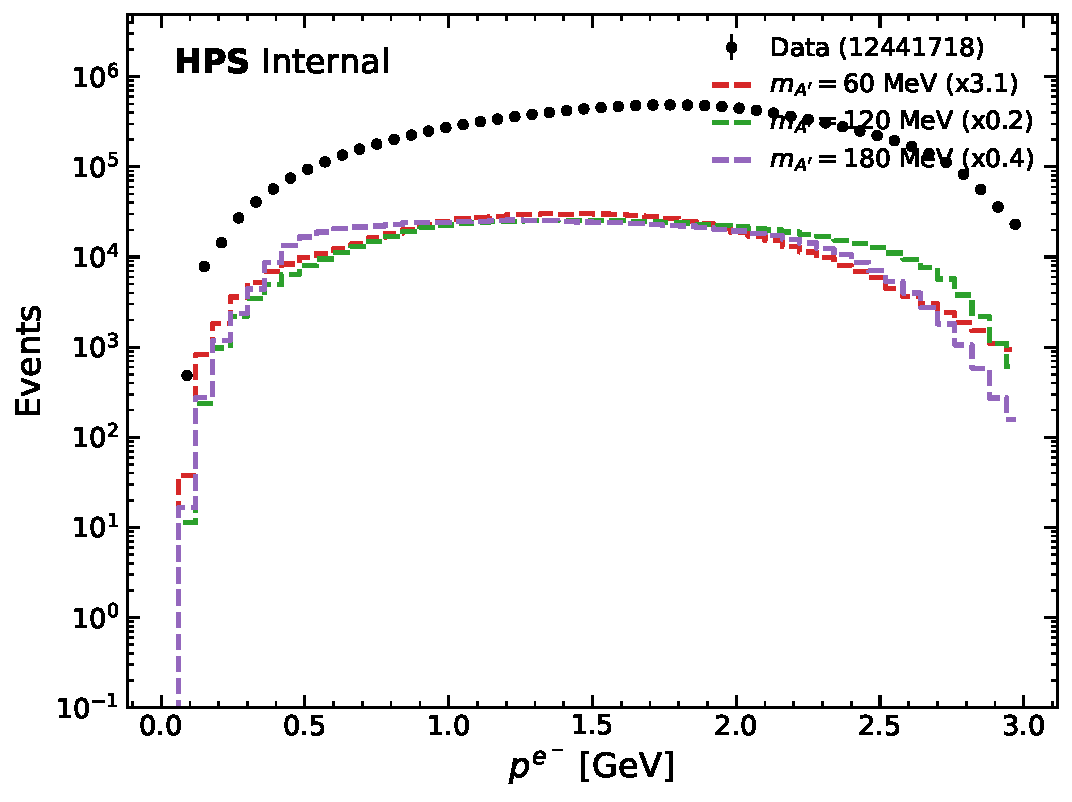
\includegraphics[width=\textwidth]{preselection_plots/signal_overlay_loose_loose_ele_p.pdf}
    \caption{Electron momentum $p$.}
  \end{subfigure}\hfill
  \begin{subfigure}[t]{0.48\textwidth}
    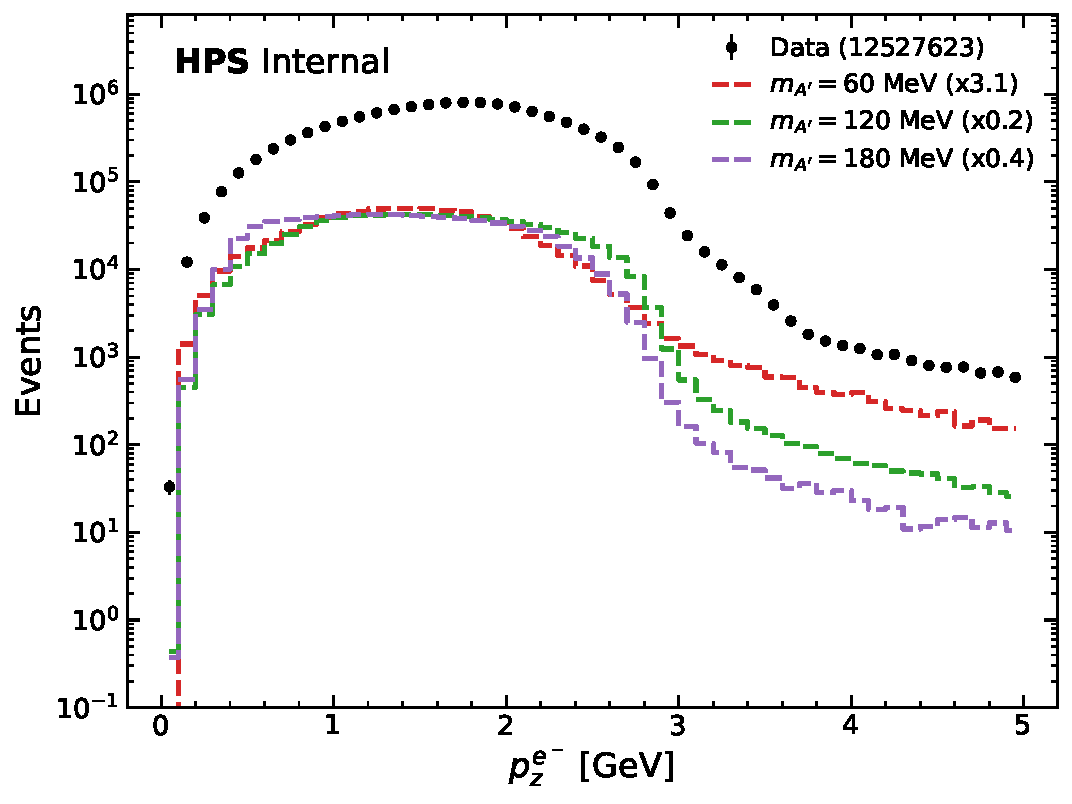
\includegraphics[width=\textwidth]{preselection_plots/signal_overlay_loose_loose_ele_pz.pdf}
    \caption{Electron longitudinal momentum $p_z$.}
  \end{subfigure}

  \vspace{0.5em}
  \begin{subfigure}[t]{0.48\textwidth}
    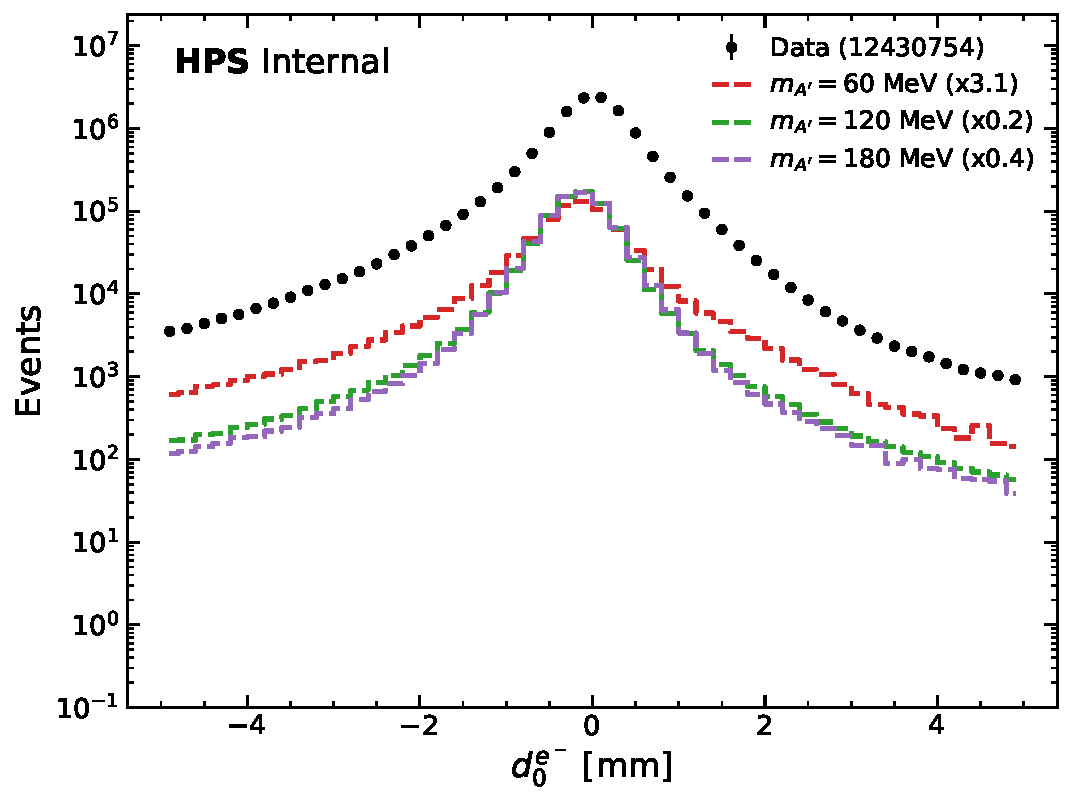
\includegraphics[width=\textwidth]{preselection_plots/signal_overlay_loose_loose_ele_d0.pdf}
    \caption{Electron transverse impact parameter $d_0$.}
  \end{subfigure}\hfill
  \begin{subfigure}[t]{0.48\textwidth}
    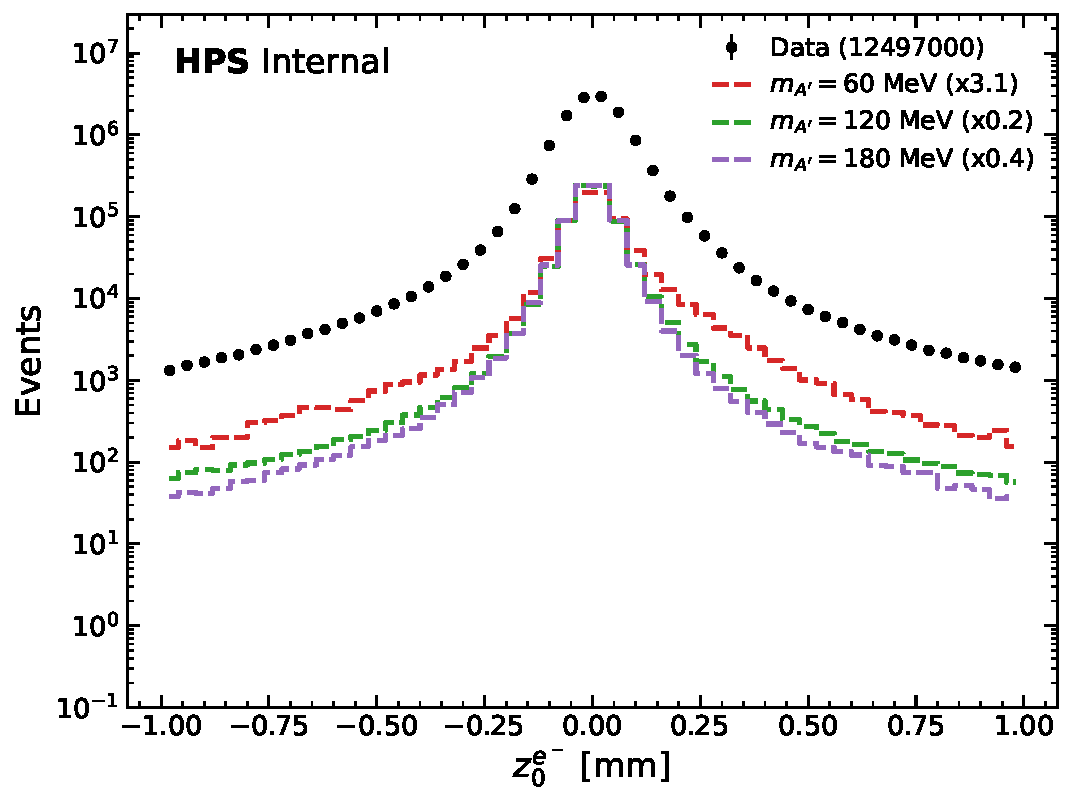
\includegraphics[width=\textwidth]{preselection_plots/signal_overlay_loose_loose_ele_z0.pdf}
    \caption{Electron longitudinal impact parameter $z_0$.}
  \end{subfigure}
  \caption{Electron-track kinematic distributions after the loose preselection,
    comparing data (points) with the signal MC (filled histogram).}
  \label{fig:presel_ele_kin}
\end{figure}

% ------------------------------------------------------------
%  2. Positron track kinematics
% ------------------------------------------------------------
% Figure~\ref{fig:presel_pos_kin} shows the corresponding positron-track
% quantities. As for the electron, the momentum and impact-parameter
% distributions are used to validate the modelling of the reconstructed final
% state prior to any signal-region selection.
\begin{figure}[htbp]
  \centering
  \begin{subfigure}[t]{0.48\textwidth}
    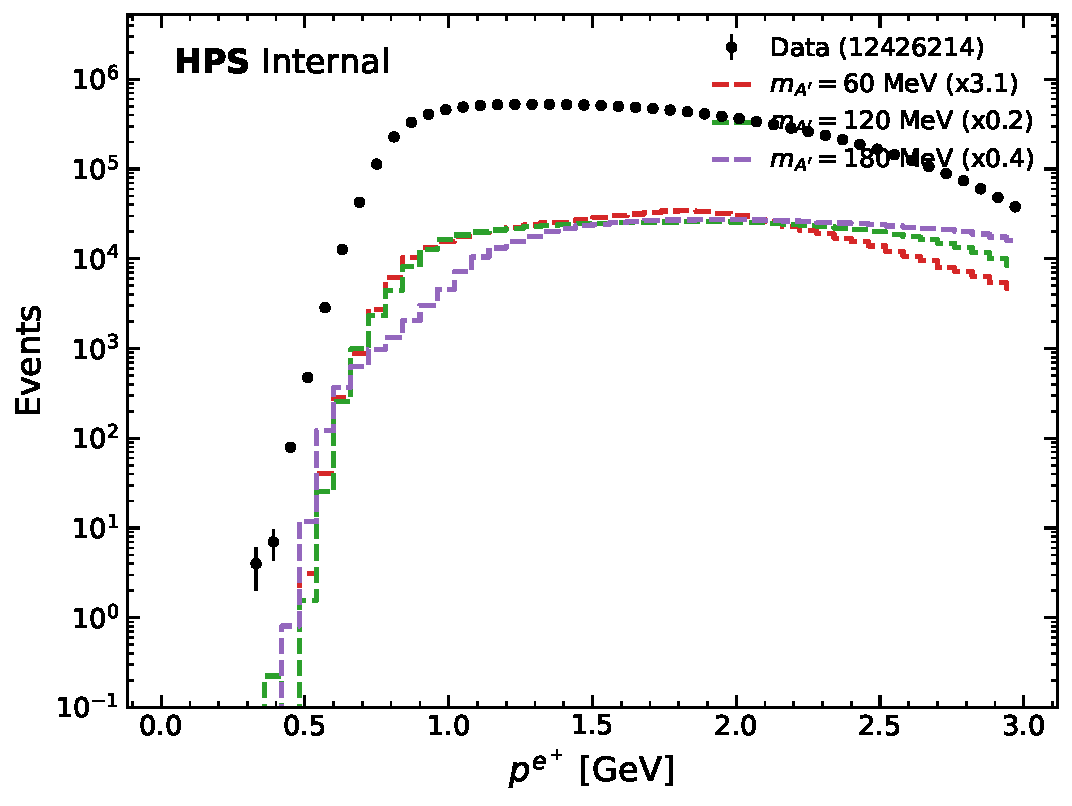
\includegraphics[width=\textwidth]{preselection_plots/signal_overlay_loose_loose_pos_p.pdf}
    \caption{Positron momentum $p$.}
  \end{subfigure}\hfill
  \begin{subfigure}[t]{0.48\textwidth}
    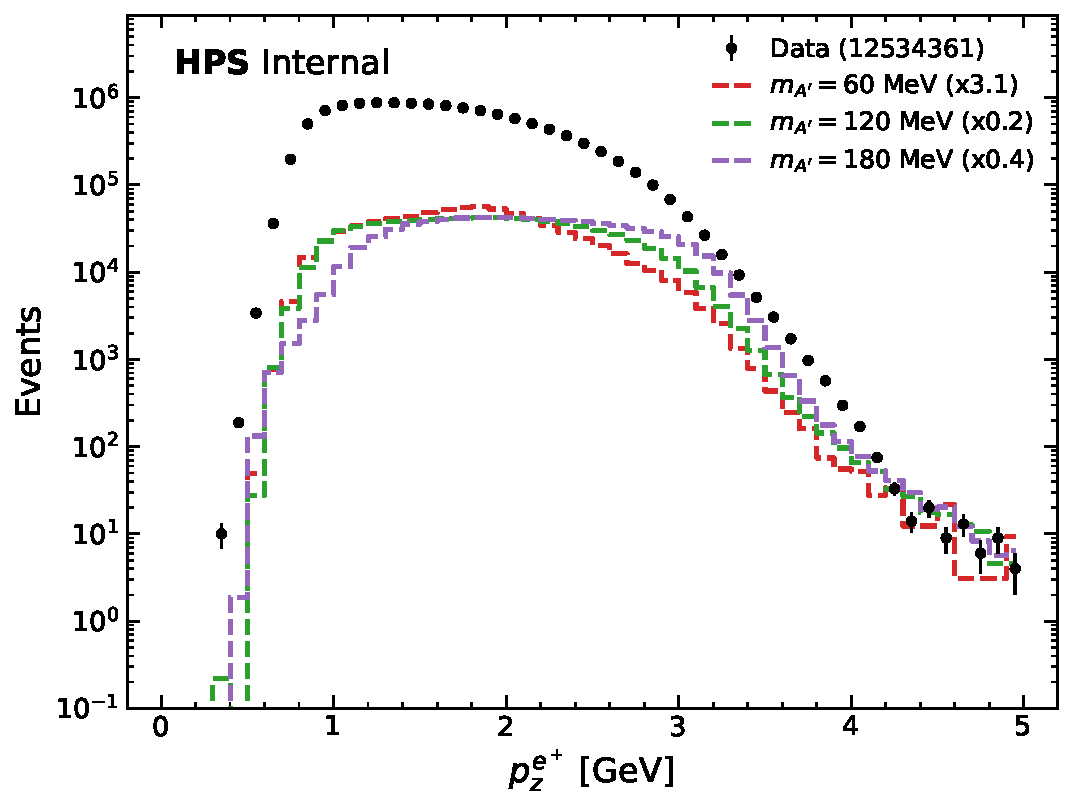
\includegraphics[width=\textwidth]{preselection_plots/signal_overlay_loose_loose_pos_pz.pdf}
    \caption{Positron longitudinal momentum $p_z$.}
  \end{subfigure}

  \vspace{0.5em}
  \begin{subfigure}[t]{0.48\textwidth}
    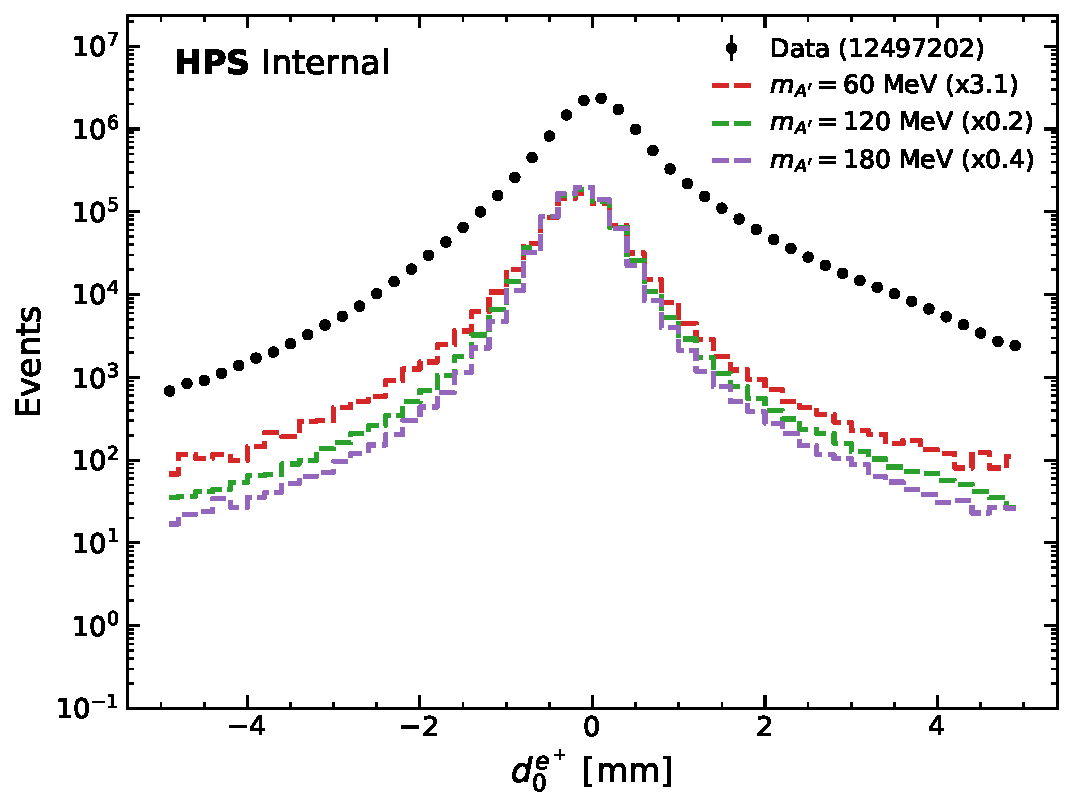
\includegraphics[width=\textwidth]{preselection_plots/signal_overlay_loose_loose_pos_d0.pdf}
    \caption{Positron transverse impact parameter $d_0$.}
  \end{subfigure}\hfill
  \begin{subfigure}[t]{0.48\textwidth}
    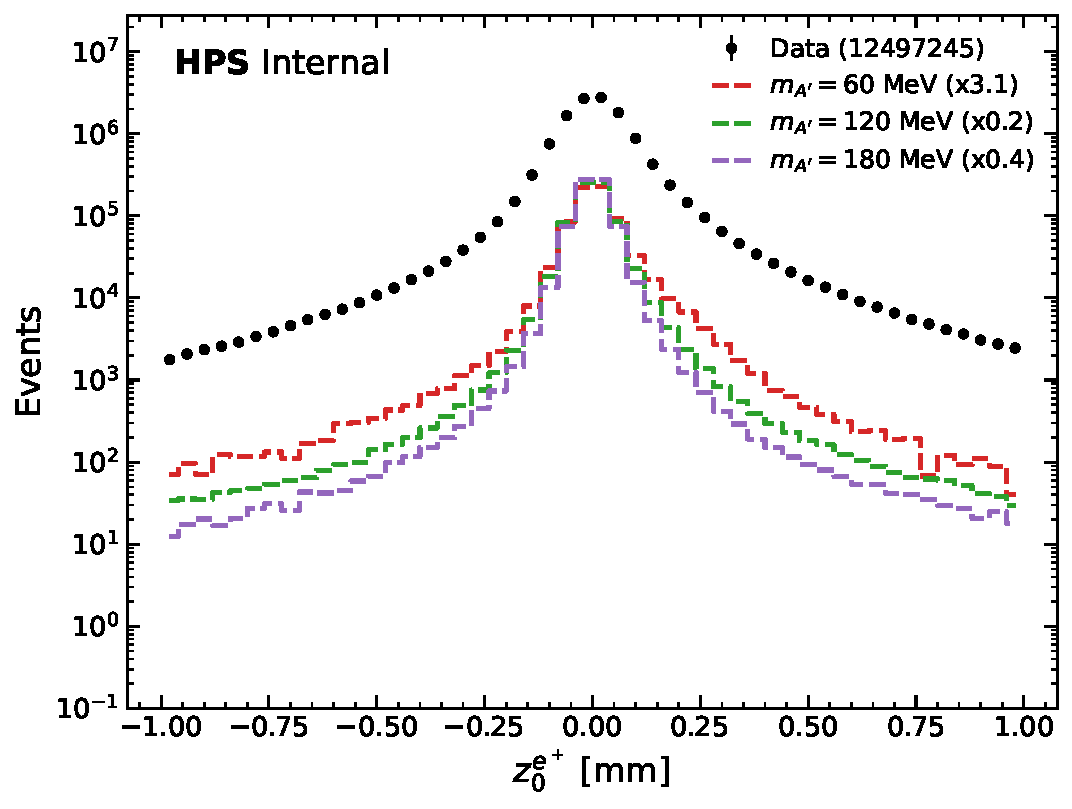
\includegraphics[width=\textwidth]{preselection_plots/signal_overlay_loose_loose_pos_z0.pdf}
    \caption{Positron longitudinal impact parameter $z_0$.}
  \end{subfigure}
  \caption{Positron-track kinematic distributions after the loose preselection,
    comparing data (points) with the signal MC (filled histogram).}
  \label{fig:presel_pos_kin}
\end{figure}



% ------------------------------------------------------------
%  5. Two-dimensional mass correlations
% ------------------------------------------------------------
% The two-dimensional distributions of the reconstructed invariant mass versus
% the preselection variables are shown for data (left column) and signal MC
% (right column) in the following figures. These correlations are used to check
% that the mass reconstruction is unbiased across the relevant phase space and
% that no artificial structure is introduced by the selection.
% Figure~\ref{fig:scatter_mom} shows the mass-versus-momentum correlations.
\begin{figure}[htbp]
  \centering
  \begin{subfigure}[t]{0.48\textwidth}
    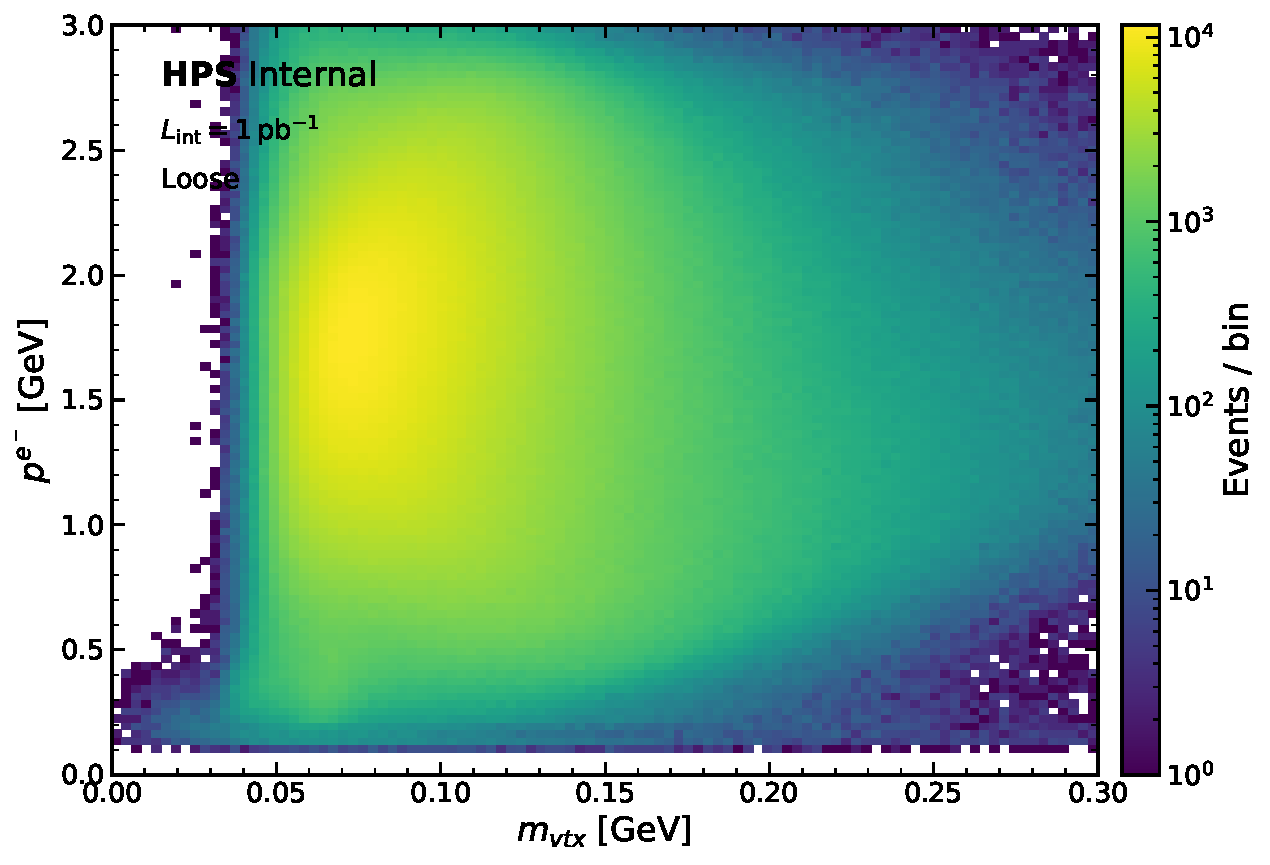
\includegraphics[width=\textwidth]{preselection_plots/xy_scatter_xy_mass_vs_ele_p_data_loose.pdf}
    \caption{Mass vs.\ electron $p$ (data).}
  \end{subfigure}\hfill
  \begin{subfigure}[t]{0.48\textwidth}
    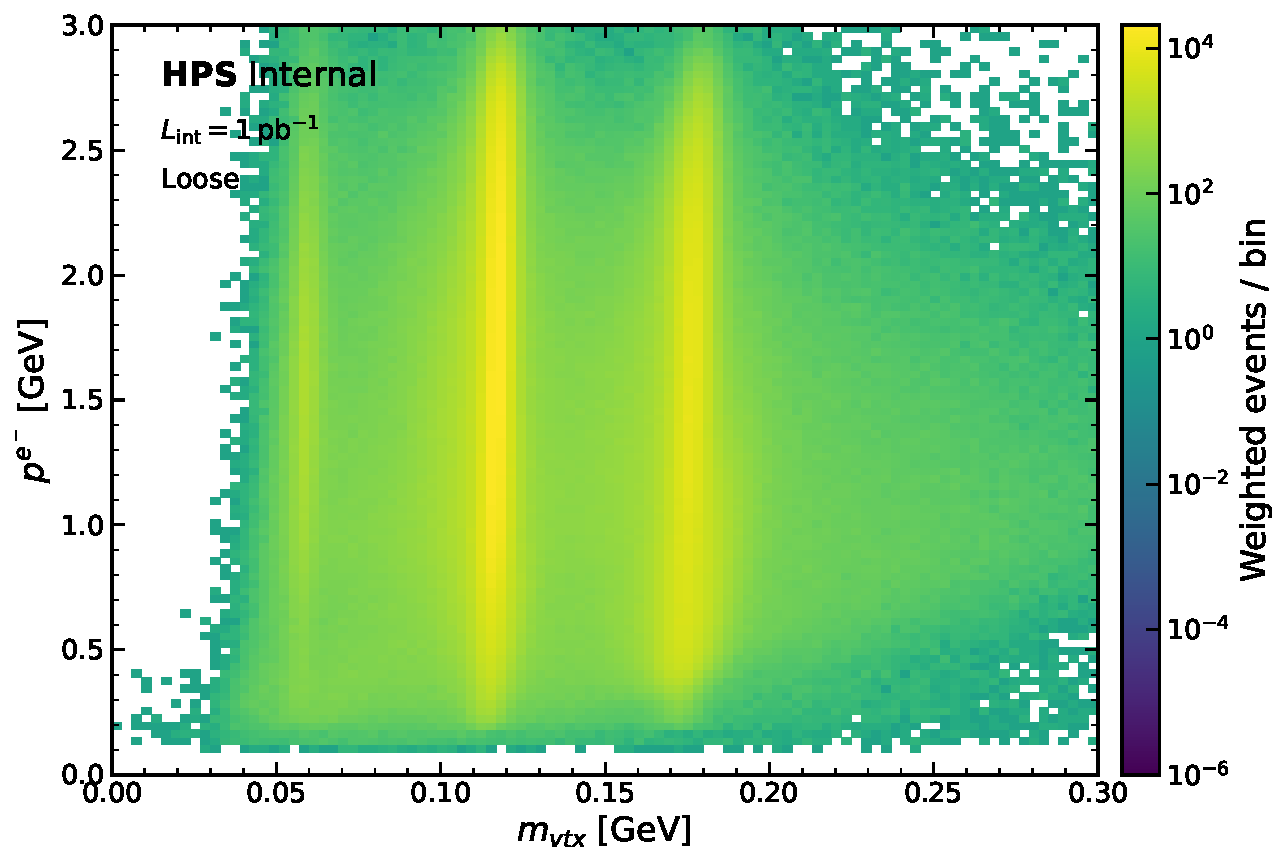
\includegraphics[width=\textwidth]{preselection_plots/xy_scatter_xy_mass_vs_ele_p_signal_loose.pdf}
    \caption{Mass vs.\ electron $p$ (signal).}
  \end{subfigure}

  \vspace{0.5em}
  \begin{subfigure}[t]{0.48\textwidth}
    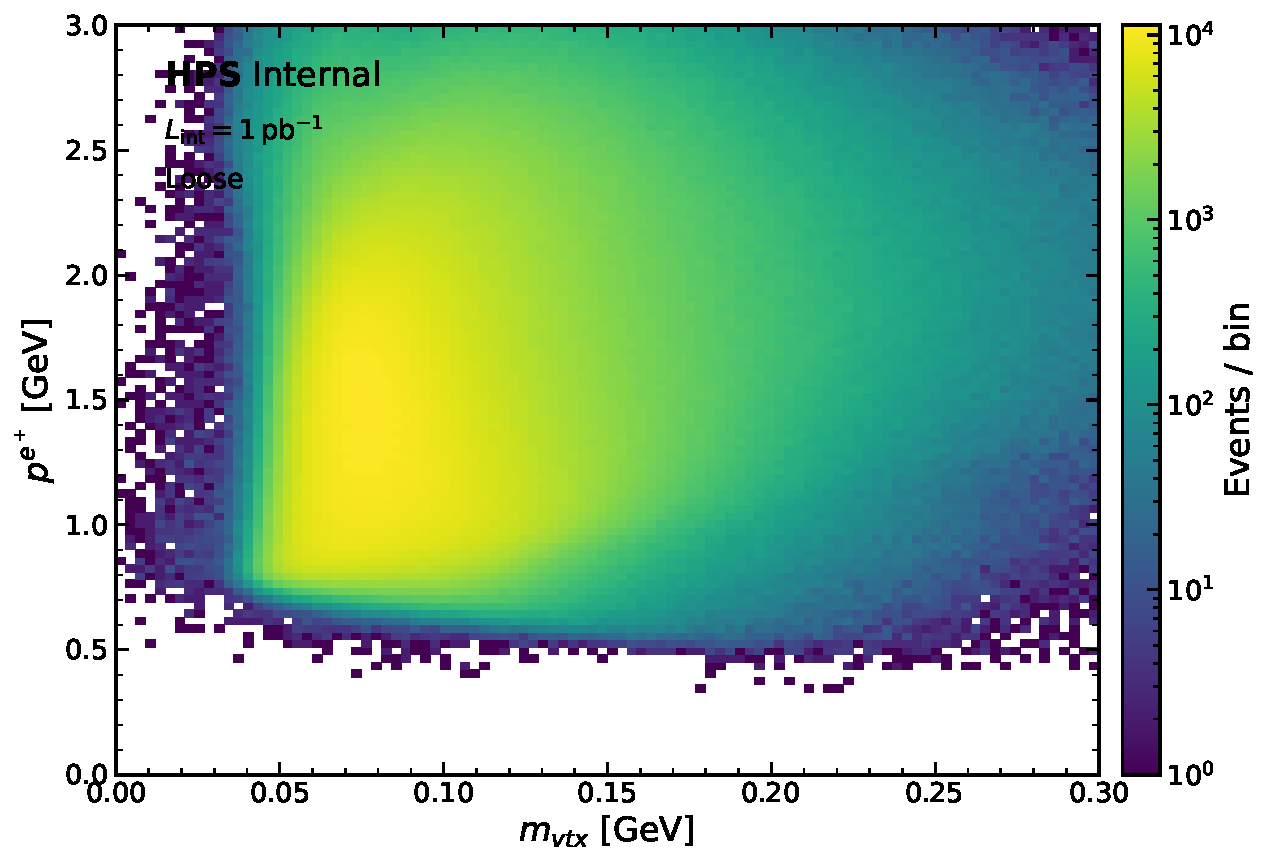
\includegraphics[width=\textwidth]{preselection_plots/xy_scatter_xy_mass_vs_pos_p_data_loose.pdf}
    \caption{Mass vs.\ positron $p$ (data).}
  \end{subfigure}\hfill
  \begin{subfigure}[t]{0.48\textwidth}
    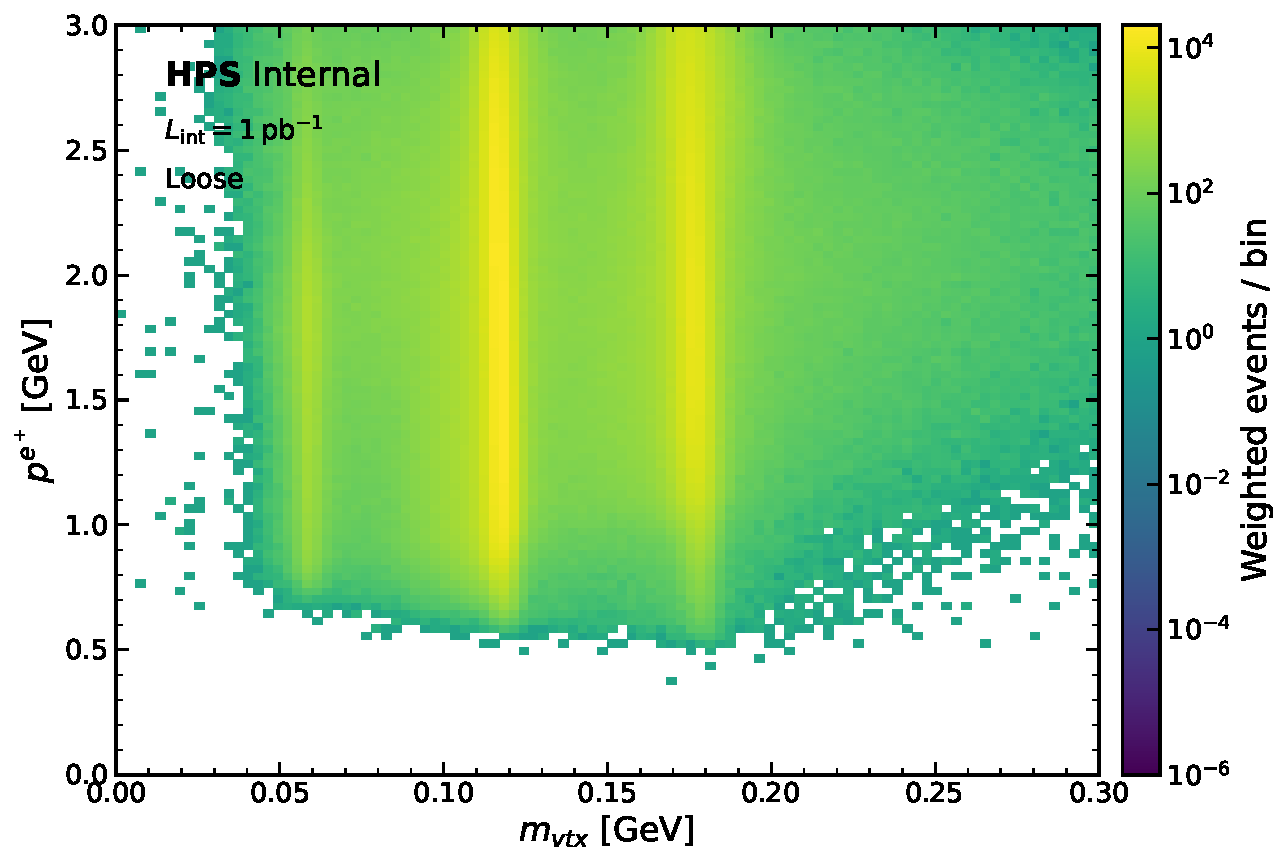
\includegraphics[width=\textwidth]{preselection_plots/xy_scatter_xy_mass_vs_pos_p_signal_loose.pdf}
    \caption{Mass vs.\ positron $p$ (signal).}
  \end{subfigure}

  \caption{Reconstructed invariant mass versus momentum observables, for data
    (left) and signal MC (right), after the loose preselection.}
  \label{fig:scatter_mom}
\end{figure}

% Figure~\ref{fig:scatter_chi2} shows the mass-versus-track/vertex-quality
% correlations.
\begin{figure}[htbp]
  \centering
  \begin{subfigure}[t]{0.48\textwidth}
    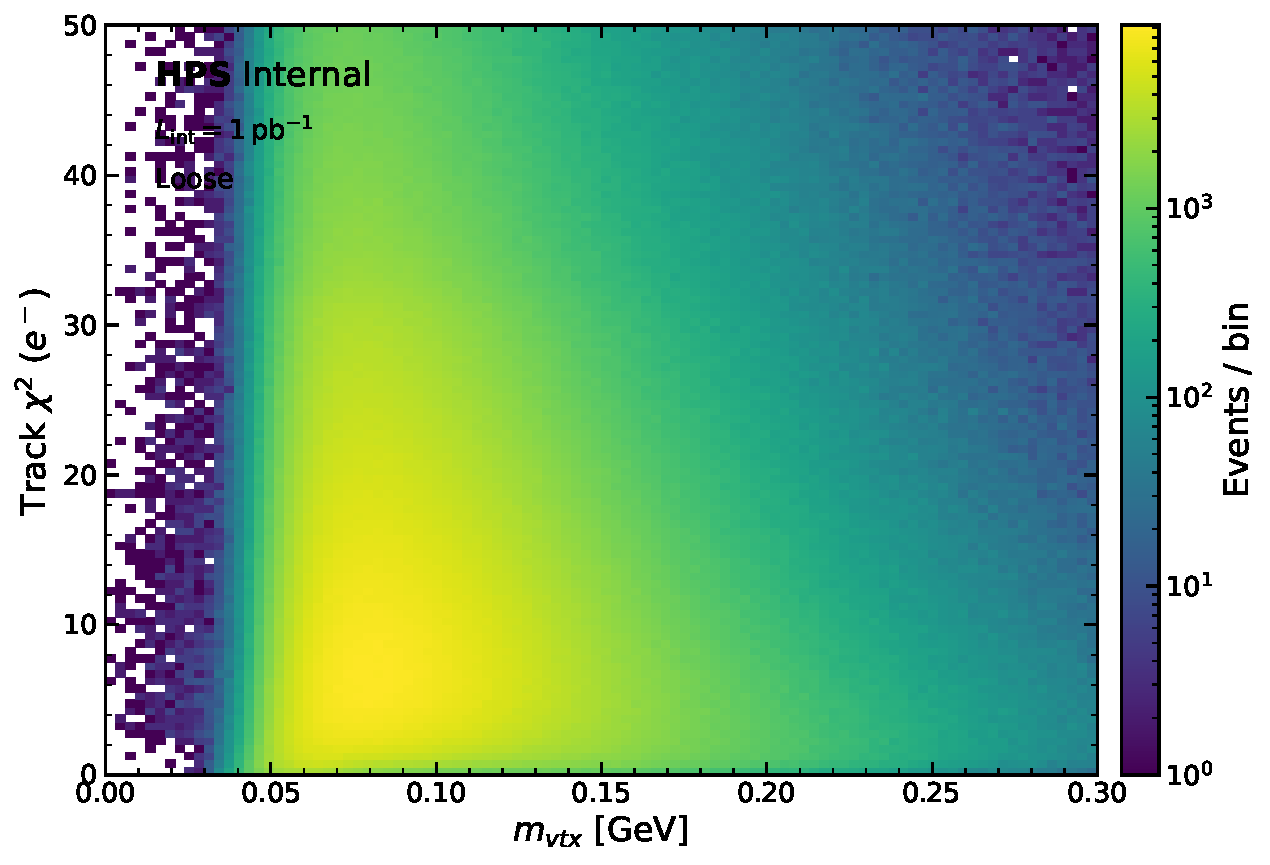
\includegraphics[width=\textwidth]{preselection_plots/xy_scatter_xy_mass_vs_ele_chi2_data_loose.pdf}
    \caption{Mass vs.\ electron $\chi^2$ (data).}
  \end{subfigure}\hfill
  \begin{subfigure}[t]{0.48\textwidth}
    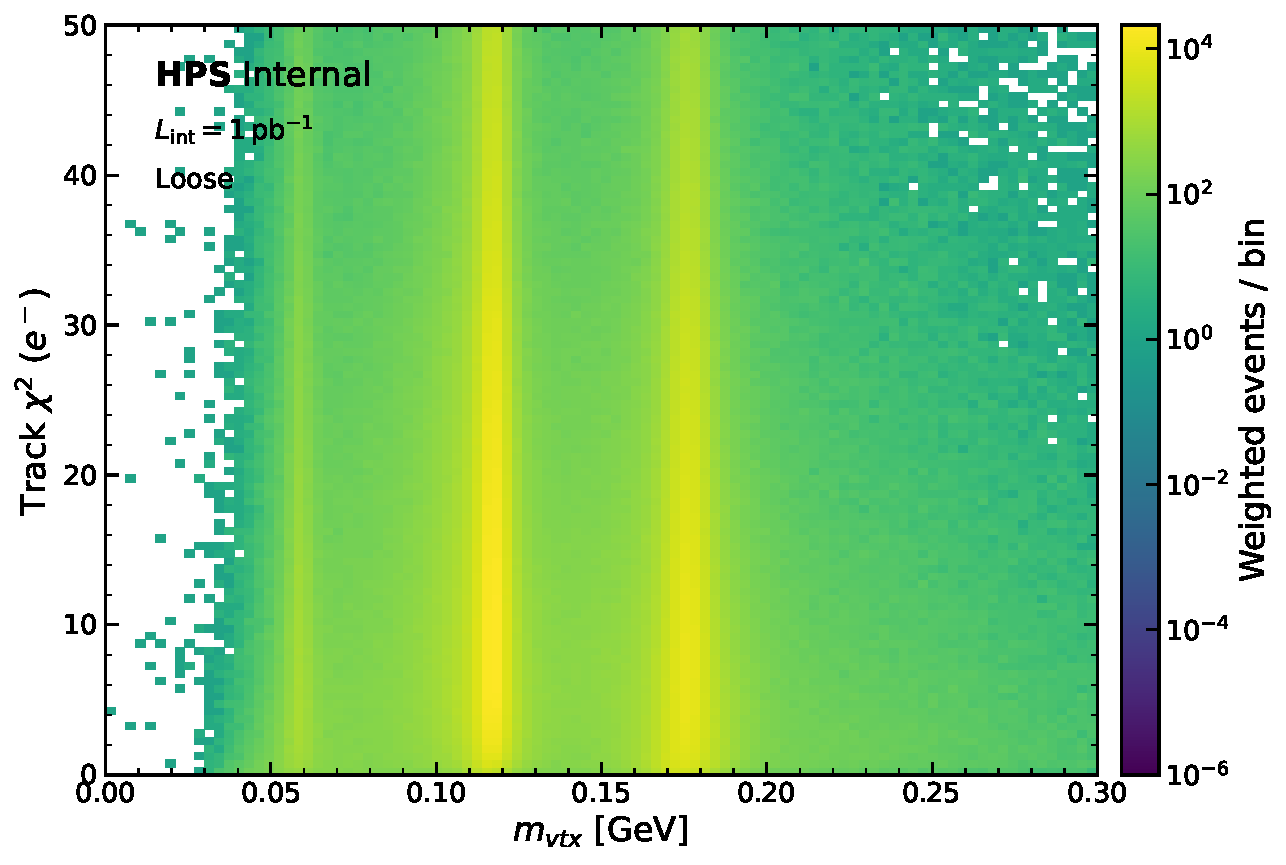
\includegraphics[width=\textwidth]{preselection_plots/xy_scatter_xy_mass_vs_ele_chi2_signal_loose.pdf}
    \caption{Mass vs.\ electron $\chi^2$ (signal).}
  \end{subfigure}

  \vspace{0.5em}
  \begin{subfigure}[t]{0.48\textwidth}
    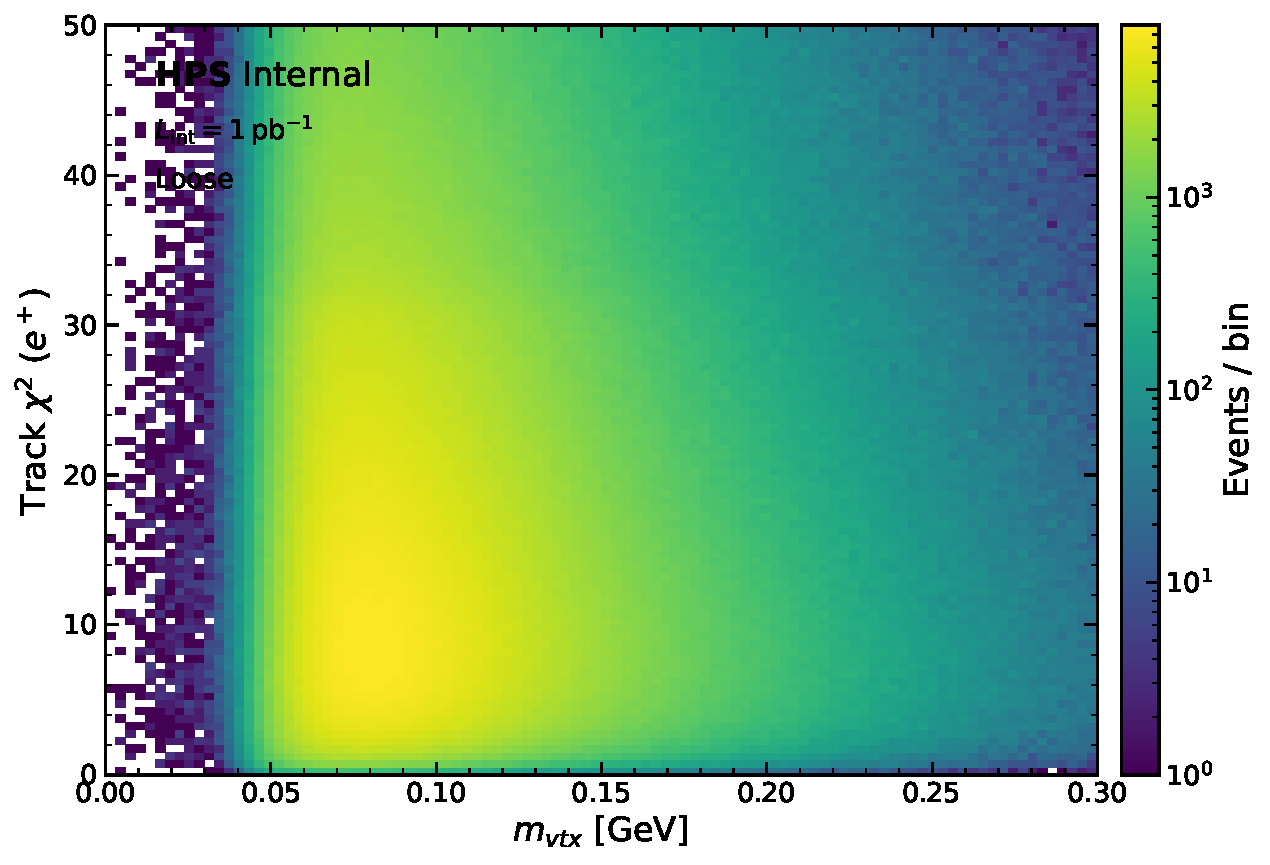
\includegraphics[width=\textwidth]{preselection_plots/xy_scatter_xy_mass_vs_pos_chi2_data_loose.pdf}
    \caption{Mass vs.\ positron $\chi^2$ (data).}
  \end{subfigure}\hfill
  \begin{subfigure}[t]{0.48\textwidth}
    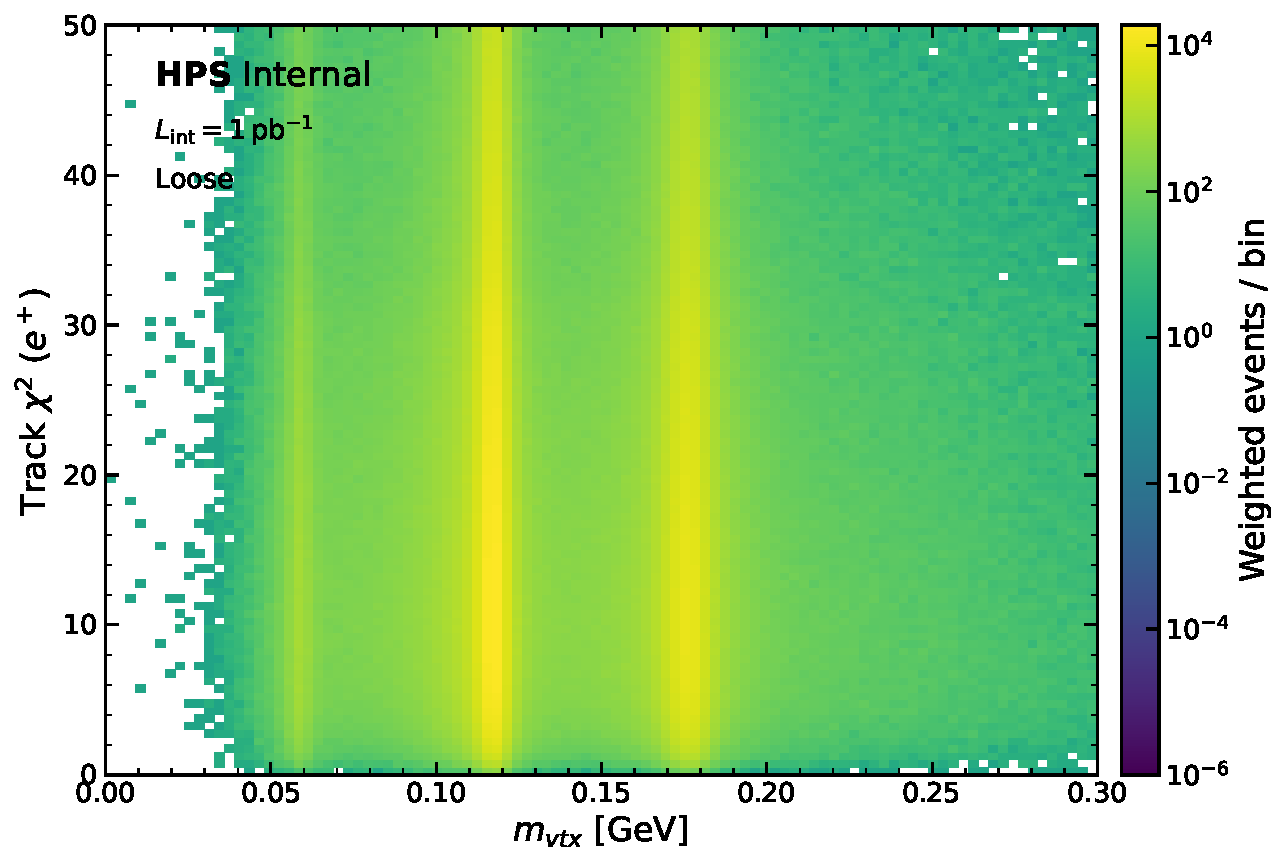
\includegraphics[width=\textwidth]{preselection_plots/xy_scatter_xy_mass_vs_pos_chi2_signal_loose.pdf}
    \caption{Mass vs.\ positron $\chi^2$ (signal).}
  \end{subfigure}

  \vspace{0.5em}
  \begin{subfigure}[t]{0.48\textwidth}
    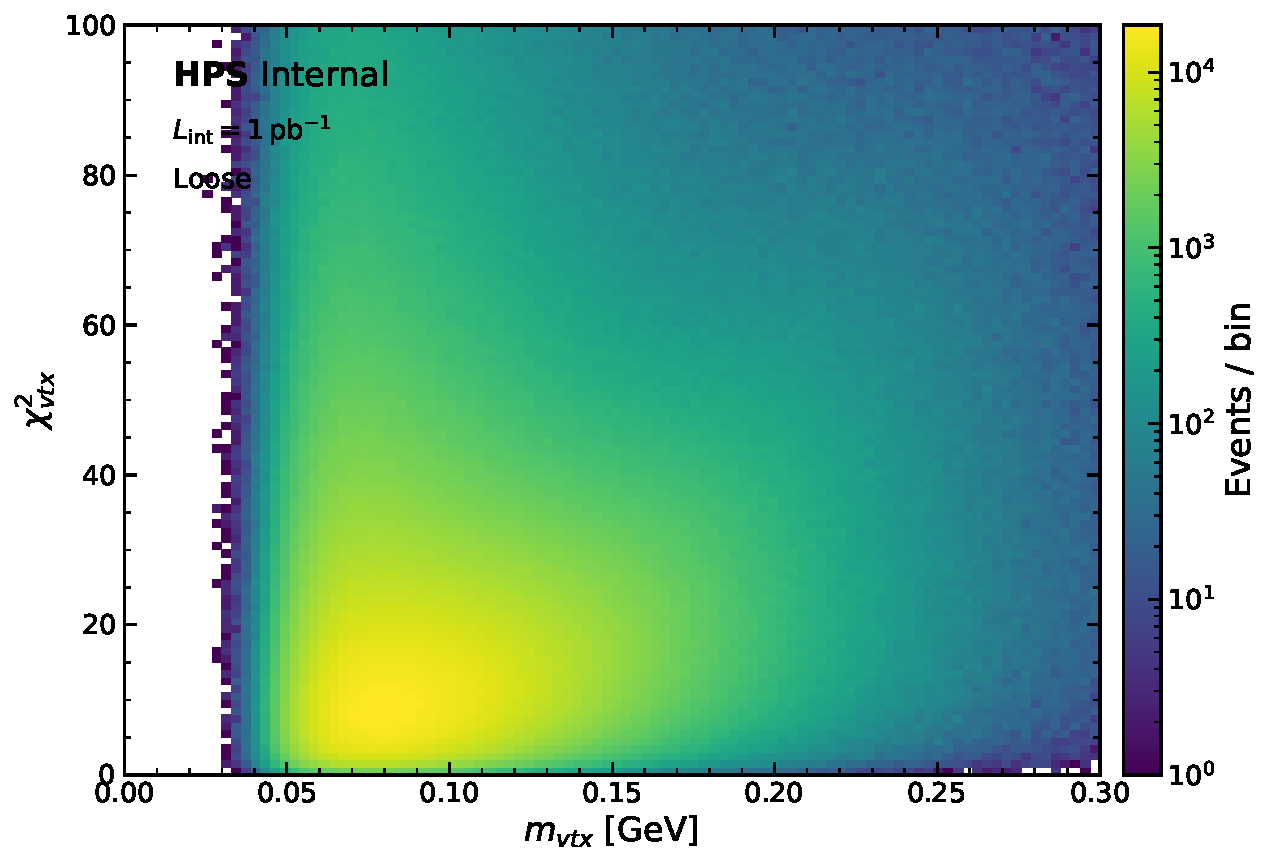
\includegraphics[width=\textwidth]{preselection_plots/xy_scatter_xy_mass_vs_vtx_chi2_data_loose.pdf}
    \caption{Mass vs.\ vertex $\chi^2$ (data).}
  \end{subfigure}\hfill
  \begin{subfigure}[t]{0.48\textwidth}
    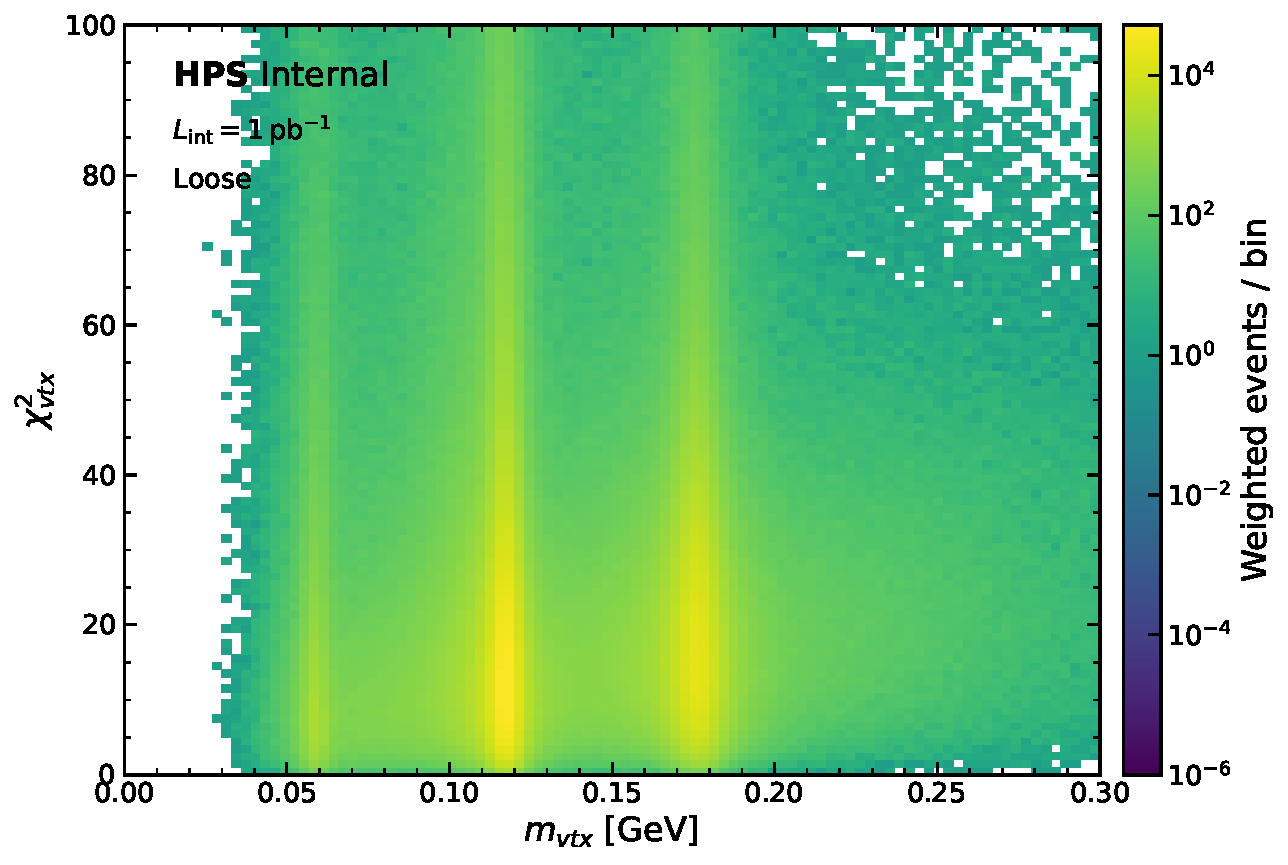
\includegraphics[width=\textwidth]{preselection_plots/xy_scatter_xy_mass_vs_vtx_chi2_signal_loose.pdf}
    \caption{Mass vs.\ vertex $\chi^2$ (signal).}
  \end{subfigure}
  \caption{Reconstructed invariant mass versus track- and vertex-fit quality,
    for data (left) and signal MC (right), after the loose preselection.}
  \label{fig:scatter_chi2}
\end{figure}

\fi

\subsection{2015 mass resolution}
\label{sec:massres-2015}

The 2015 signal width is calibrated with M{\o}ller data and propagated across mass
with simulated $A^\prime$ samples \cite{HPS2015InternalNote}. The M{\o}ller peak fixes
the detector resolution at a known mass, and the data--MC momentum-resolution
difference determines the additional smearing applied to the simulation. Rescaling
the fitted $A^\prime$ widths to that data anchor gives
\begin{equation}
\sigma_{2015}(m) = -9.22\times10^{-5} + 5.322\times10^{-2}\,m,
\label{eq:sigma2015}
\end{equation}
with $m$ and $\sigma_{2015}$ expressed in GeV.

The M{\o}ller measurement supplies the absolute response, while the simulated mass
grid supplies its mass dependence. The associated uncertainty therefore reflects the
M{\o}ller calibration, the target position, and the residual momentum-response
mismodelling \cite{HPS2015DarkPhoton,HPS2015InternalNote}. At each test mass this curve
sets both the Gaussian signal width and the width of the excluded training interval.

\begin{figure}[H]
\centering
\graphicorplaceholder{0.82\linewidth}{resolution_figs/hps2015_mass_resolution_internal_fig24.png}
\caption{2015 mass-resolution parameterization from scaled $A^\prime$ MC and M{\o}ller
data \cite{HPS2015InternalNote}. The M{\o}ller point anchors the absolute detector
response in data, while the scaled $A^\prime$ simulation supplies the mass dependence
across the search window. Because the prompt dark-photon width is negligible, this
curve directly sets the resonance width assumed in the search and therefore the local
background entering the limit.}
\label{fig:2015-resolution}
\end{figure}

\subsection{2016 mass resolution}
\label{sec:massres-2016}

The 2016 calibration follows the same strategy over a broader mass range
\cite{HPS2016BumpInternal,HPS2016PromptLong}. M{\o}ller events fix the absolute
response at \SI{48.5}{MeV}; full-energy-electron momentum peaks determine the extra
smearing needed to match data; and smeared $A^\prime$ samples carry that calibration
across the search range. A fourth-order polynomial fit to those samples defines the
2016 signal model,
\begin{align}
\sigma_{2016}(m) &= 3.8\times10^{-4} + 4.1\times10^{-2}m - 2.7\times10^{-1}m^2 \nonumber\\
&\quad + 3.49\,m^3 - 11.11\,m^4,
\qquad m \le \SI{0.18}{GeV},
\label{eq:sigma2016}
\end{align}
Earlier extended-range studies continued the polynomial linearly above
$m_0=\SI{0.18}{GeV}$ with slope \num{0.0239} to avoid its high-mass turnover. The
present 2016 scan ends at \SI{180}{MeV}, close to the published \SIrange{39}{179}{MeV}
interval, so that continuation is not used. The 2015 scan similarly remains near its
published \SIrange{19}{81}{MeV} interval, with only the upper endpoint extended to
\SI{90}{MeV}.

The smearing correction reconciles the M{\o}ller and simulated $A^\prime$ widths with
the observed tracking response \cite{HPS2016BumpInternal,HPS2016PromptLong}. Because
the resolution worsens with mass, both the signal template and the excluded training
window broaden, increasing the prompt background beneath a narrow signal hypothesis.

\begin{figure}[H]
\centering
\graphicorplaceholder{0.82\linewidth}{resolution_figs/hps2016_mass_resolution_internal_fig29.png}
\caption{2016 smeared-$A^\prime$ and M{\o}ller-based mass-resolution summary
\cite{HPS2016BumpInternal}. The smeared $A^\prime$ points show how the data-driven
momentum-smearing correction is propagated away from the single M{\o}ller calibration
point. The worsening resolution with mass broadens the signal window and is one of the
main detector effects limiting prompt sensitivity at higher mass.}
\label{fig:2016-resolution}
\end{figure}

\subsection{2021 mass resolution}
\label{sec:massres-2021}

The upgraded 2019/2021 tracker requires a separate resolution parameterization. We use
the inclusive target-constrained V0 fit without hit requirements shown in
Figure~\ref{fig:2021-resolution}. Before the final data--MC broadening, the red curve is
\begin{equation}
\sigma_{2021}^{\mathrm{TC,raw}}(m_{\mathrm{MeV}})
= \left(1.4786 - 1.1\times10^{-3}m_{\mathrm{MeV}}
  + 6.87\times10^{-5}m_{\mathrm{MeV}}^2\right)\,\mathrm{MeV},
\label{eq:sigma2021}
\end{equation}
where $m_{\mathrm{MeV}}$ is the numerical mass value in MeV. The analysis then applies the
target-constrained data/MC scale derived from the 2021 smearing study,
\begin{equation}
s_{\mathrm{TC}} = \frac{2.186}{1.745} \simeq 1.25,
\qquad
\sigma_{2021}^{\mathrm{TC,smear}}(m)
= s_{\mathrm{TC}}\,\sigma_{2021}^{\mathrm{TC,raw}}(m).
\label{eq:sigma2021-tc-smear}
\end{equation}
The scale comes from the target-constrained row after hit and curvature ($\Omega$)
smearing are applied to the simulation. Equation~\ref{eq:sigma2021-tc-smear} then sets
the 2021 signal width and the corresponding excluded training interval at each mass.

\begin{figure}[H]
\centering
\graphicorplaceholder{0.78\linewidth}{resolution_figs/hps2021_mass_resolution_target_constrained_nohitreq.png}
\caption{2021 mass-resolution summary used for the prompt analysis. The red curve is
the inclusive target-constrained V0 quadratic fit without hit requirements before the
TC data/MC broadening in Eq.~\ref{eq:sigma2021-tc-smear}. The blue curve shows the
corresponding unconstrained V0 reference fit included in the underlying study for
comparison.}
\label{fig:2021-resolution}
\end{figure}

\begin{figure}[H]
\centering
\graphicorplaceholder{0.78\linewidth}{resolution_figs/hps2021_data_mc_smearing_scale.png}
\caption{2021 M{\o}ller run data/MC mass-resolution comparison used to set the
smearing scale.
Here UC denotes the unconstrained vertex sample, BSC denotes the beamspot-constrained
vertex sample, and TC denotes the target-constrained vertex sample. The TC row is the
most relevant row for the prompt analysis; comparing the data value
\SI{2.186}{MeV} to the $\Omega$+hit-smeared Monte Carlo value \SI{1.745}{MeV}
gives the applied scale factor $2.186/1.745\simeq1.25$.}
\label{fig:2021-data-mc-smearing-scale}
\end{figure}

Figure~\ref{fig:mass-resolution-three-panel} compares the three resolution curves used
to construct the signal templates and excluded training windows over their respective
scan ranges.

\begin{figure}[H]
\centering
\graphicorplaceholder{0.78\linewidth}{resolution_figs/hps_mass_resolution_three_panel.png}
\caption{Mass-resolution parameterizations used by the analysis over the adopted
scan ranges. The 2016 scan ends at the polynomial boundary of \SI{180}{MeV}, so its
configured high-mass continuation is not used. The 2021 panel shows the target-constrained V0 parameterization after
multiplication by the TC smearing scale $s_{\mathrm{TC}}=2.186/1.745\simeq1.25$ and
extended to \SI{250}{MeV}.}
\label{fig:mass-resolution-three-panel}
\end{figure}

\subsection{Radiative fraction and the \texorpdfstring{$\eps^2$}{epsilon2} normalization}
\label{sec:radfrac}

The radiative fraction encodes the fraction of the selected prompt background arising
from the purely radiative trident process,
\begin{equation}
f_{\mathrm{rad},d}(m)
=
\frac{dN_{\gamma^\ast,d}/dm}{dN_{\mathrm{tri},d}/dm + dN_{\mathrm{wab},d}/dm},
\label{eq:frad-def}
\end{equation}
where the numerator is the selected radiative-trident component and the denominator is
the full selected prompt background for dataset $d$
\cite{HPS2015DarkPhoton,HPS2016PromptLong}. Because heavy-photon production is
normalized to the radiative trident rate, $f_{\mathrm{rad}}$ is the physics quantity
that converts a fitted prompt signal yield into a limit on the coupling. With this
notation,
\begin{equation}
K_d(m) \equiv A_d(\eps^2 = 1)
= \frac{3\pi\,m\,f_{\mathrm{rad},d}(m)\,\rho_d(m)}{2\alpha_{\mathrm{EM}}},
\qquad
A_d = K_d(m)\,\eps^2,
\label{eq:kd-radfrac}
\end{equation}
where $\rho_d(m)$ is the selected prompt-spectrum density in dataset $d$. The
engineering-run inputs follow the corresponding prompt searches, while the 2021
normalization remains provisional for the native 10\% sample.

\subsubsection{2015 radiative fraction}

The 2015 prompt search used a constant approximation,
\begin{equation}
f_{\mathrm{rad},2015}(m) = 0.085,
\end{equation}
which the analysis retains as its 2015 baseline. The dedicated 2015
radiative-fraction study compares the selected radiative-trident component with the
total prompt background and adopts the red horizontal line at 8.5\% as a conservative
description across the search interval. The constant comes from the internal HPS
normalization study rather than from the GP fit and is retained for consistency with
the published 2015 analysis.

\begin{figure}[H]
\centering
\graphicorplaceholder{0.96\linewidth}{normalization_figs/hps2015_radiative_fraction_review.png}
\caption{Dedicated 2015 radiative-fraction inputs. The left panel shows the selected
cross-section composition, while the right panel shows the radiative fraction used for
normalization. The red horizontal line denotes the 8.5\% constant adopted as the
conservative fit across the 2015 prompt-search dataset. This quantity converts the
measured prompt spectrum into the expected $A^\prime$ normalization, so it affects the
final $\eps^2$ interpretation rather than the local spectral fit itself.}
\label{fig:2015-radfrac}
\end{figure}

\subsubsection{2016 radiative fraction}

The 2016 prompt search used a fifth-order polynomial derived from radiative, trident,
and converted-WAB MC after the full prompt selection. Those components determine the
mass-dependent conversion from fitted signal yield to $\eps^2$ over the 2016 search
range. For the 2016 input, we instead use the constant approximation
\begin{equation}
f_{\mathrm{rad},2016}(m) = 0.05,
\end{equation}
which is numerically stable over the wider scan range. Figure~\ref{fig:2016-radfrac}
shows the mass-dependent simulation used in the published determination; the constant
used here is a working numerical approximation to that richer model.

\begin{figure}[H]
\centering
\graphicorplaceholder{0.82\linewidth}{normalization_figs/hps2016_radiative_fraction_internal_fig30.png}
\caption{2016 radiative-fraction study from radiative, trident, and converted-WAB MC
\cite{HPS2016BumpInternal}. The simulation gives an intrinsically mass-dependent
normalization, although this analysis uses the constant
$f_{\mathrm{rad},2016}=0.05$ for numerical stability.}
\label{fig:2016-radfrac}
\end{figure}

\subsubsection{2021 radiative fraction}

For the native 2021 10\% sample, we use the provisional value
\begin{equation}
f_{\mathrm{rad},2021}(m) = 0.05.
\end{equation}
The 2021 full analysis note constructs the ratio from selected radiative-trident,
tritrig, and WAB samples after preselection and a high-momentum requirement quoted as
$p_{\mathrm{vtx}}>2.8~\mathrm{GeV}$. A fit over
$0.05<m<0.25~\mathrm{GeV}$ gives the constant average
$f_{\mathrm{rad}}^{\mathrm{const}}=0.0496$ \cite[Sec.~6.1, Figs.~92--93,
Eqs.~25--26]{HPS2021FullAnalysisNote}. Thus 0.05 is a reasonable approximation over
most of the 2021 search range. Before it is used for a final 2021 result, this
normalization must be checked directly against the prompt-TC $p_{\mathrm{sum}}$
selection and its threshold convention; the mass-dependent parameterization provides a
useful cross-check.

\begin{figure}[H]
\centering
\graphicorplaceholder{0.82\linewidth}{normalization_figs/hps2021_radiative_fraction_note_fig92.png}
\caption{2021 selected-mass distributions used to form the radiative fraction in the
full-analysis note \cite{HPS2021FullAnalysisNote}. The upper panel shows the selected
radiative, tritrig, and WAB components, while the lower panel gives
$f_{\mathrm{rad}}(m)=N_{\mathrm{rad}}/N_{\mathrm{bkg}}$.}
\label{fig:2021-radfrac-note-components}
\end{figure}

\begin{figure}[H]
\centering
\graphicorplaceholder{0.72\linewidth}{normalization_figs/hps2021_radiative_fraction_note_fig93.png}
\caption{Fifth-order 2021 full-analysis-note fit to the binned radiative fraction
\cite{HPS2021FullAnalysisNote}. The fitted curve is close to the constant value
$0.05$ across most of the range used by the 2021 analysis.}
\label{fig:2021-radfrac-note-fit}
\end{figure}

\subsection{Systematic penalties from the radiative fraction}
\label{sec:radfrac-penalty}

The analysis applies a data-set-dependent radiative-fraction penalty,
\begin{equation}
f_{\mathrm{rad},d}^{\mathrm{eff}}(m)
= \left(1-\delta_{f,d}\right) f_{\mathrm{rad},d}(m).
\label{eq:frad-penalty}
\end{equation}
The penalty enters only when signal yield is converted to $\eps^2$. It changes the
normalization of the inferred coupling without altering the blind-window likelihood.

The nominal configuration uses
\begin{equation}
(\delta_{f,2015},\delta_{f,2016},\delta_{f,2021})=(0.070,0.070,0.046).
\label{eq:frad-penalty-vector}
\end{equation}
For a fixed signal-yield limit, these shifts weaken the coupling-squared limit by
factors $1/0.93$ for 2015 and 2016 and $1/0.954$ for 2021. In the combined fit each
$K_d(m)$ is reduced by its own amount, so a larger shared $\eps^2$ is required to
produce the same yields. The factors are fixed, one-sided normalization shifts; they
do not enter the GP interpolation and are not profiled as nuisance parameters.

The 7\% engineering-run penalties reflect the several-percent uncertainty in the 2015
radiative and total $e^+e^-$ composition and the corresponding 2016 uncertainty from
the selected radiative, trident, and converted-WAB inputs
\cite{HPS2015InternalNote,HPS2016PromptLong}. We retain 7\% as a conservative
first-order treatment for both engineering runs. The 2021 term uses the
upgraded-detector estimate below.

The 2021 full analysis note assigns 3.5\% from the RAD and WAB cross sections shown in
Fig.~\ref{fig:2021-radfrac-xsec-note}, using their quoted widths and the relative
normalization $R=0.244$ \cite[Sec.~9.1, Fig.~161]{HPS2021FullAnalysisNote}. It assigns a
further 3\% for preselection and radiative-fraction modeling, motivated by
WAB-selective mismodeling in the selected background
\cite[Sec.~9.2]{HPS2021FullAnalysisNote}. Treating the two terms as independent gives
\begin{equation}
\delta_{f,2021}^{\mathrm{note}}
= \sqrt{(0.035)^2 + (0.030)^2}
= 0.046,
\qquad
f_{\mathrm{rad},2021}^{\mathrm{eff}}
= 0.954\,f_{\mathrm{rad},2021}.
\label{eq:frad-2021-note-penalty}
\end{equation}
The 2015 and 2016 penalties remain at 7\%.

\begin{figure}[H]
\centering
\graphicorplaceholder{0.88\linewidth}{normalization_figs/hps2021_radiative_xsec_note_fig16.png}
\caption{Generated cross-section distributions for the 2021 tritrig, radiative, and
WAB background MC samples \cite{HPS2021FullAnalysisNote}. These distributions set the
cross-section normalization inputs for the 2021 radiative-fraction calculation.}
\label{fig:2021-radfrac-xsec-note}
\end{figure}

\begin{figure}[H]
\centering
\graphicorplaceholder{0.76\linewidth}{normalization_figs/hps2021_radiative_xsec_uncertainty_note_fig161.png}
\caption{RAD and WAB cross-section distributions used in the 2021 note's
radiative-fraction cross-section uncertainty propagation \cite{HPS2021FullAnalysisNote}.
Together with the relative normalization $R=0.244$, these inputs lead to the 3.5\%
MC cross-section contribution.}
\label{fig:2021-radfrac-xsec-syst-note}
\end{figure}

The 4.6\% term covers only the radiative-fraction normalization. The broader 2021
displaced-search uncertainty model in Fig.~\ref{fig:2021-syst-table-note} also includes
mass resolution, target position, and tight-selection effects that must be revisited
before applying it to the full data set \cite[Sec.~9,
Table~58]{HPS2021FullAnalysisNote}. Those signal-yield and acceptance uncertainties are
not included in Eq.~\eqref{eq:frad-penalty}.

\begin{figure}[H]
\centering
\graphicorplaceholder{0.62\linewidth}{normalization_figs/hps2021_systematics_note_table58.png}
\caption{Broader 2021 full-analysis-note systematic summary
\cite{HPS2021FullAnalysisNote}. Only the MC cross-section and preselection entries
are folded into the radiative-fraction-only penalty in
Eq.~\eqref{eq:frad-2021-note-penalty}; the other entries remain separate signal-yield
or acceptance effects.}
\label{fig:2021-syst-table-note}
\end{figure}

The selected spectra, resolution curves, and radiative fractions now specify the three
data-dependent ingredients of the search: the observed mass distribution, the shape of
a narrow signal, and the conversion from fitted signal yield to coupling. The next
section describes how the GP predicts the smooth background beneath each tested mass.
